\part{Conceptos avanzados}

\section{Sistemas distribuidos}

Un sistema distribuido es un conjunto de nodos conectados a través de un red de comunicación. Desde el punto de vista específico de cada nodo, el resto de los nodos y sus respectivos recursos son remotos mientras que los suyos son locales.

Hay 4 grandes razones para construir sistemas distribuidos: 

\begin{itemize}
	\item\textbf{Compartir  recursos:} Si hay varios sitios conectados entre si, entonces un usario puede usar los recursos disponibles en alguno de los nodos de la red. En general, los mecanismos para realizar esto son dispositivos de hardware especializados.
	\item\textbf{Aceleración de procesamiento:} Si hay un proceso que puede ser particionado en varias subprocesos que se pueden correr de manera concurrente, entonces un sistema distribuido puede usar distintos nodos para correrlos simultáneamente para ahorrar tiempo. Adicionalmente, si un nodo está demasiado sobrecargado, el sistema puede repartir el trabajo a otros nodos que no estén en uso (esto se llama \textbf{load sharing} o \textbf{job migration}).
	\item\textbf{Redundancia:} Los sistemas distribuidos permiten mantener copias redundantes de sus datos en distintos nodos de la red. De esta manera, si un nodo cae, un usuario puede seguir accediendo a la información que necesita sin ningún problema.
\end{itemize}

Si bien estas son buenas razones para hacer sistemas distribuidos hay que tener en cuenta que su implementación conlleva resolver ciertos problemas como:

\begin{itemize}
	\item \textbf{Sincronización de eventos:} Como ordenarlos eventos cronológicamente. En general, cada nodo de una red tiene su propio clock y es imposible que todos los clock estén sincronizados a la perfección por lo que se deben implementar mecanismos que permitan decidir si un evento en un nodo $a$ es anterior o posterior a un evento en un nodo $b$.
	\item \textbf{Coherencia de datos:} Se debe asegurar que los datos sean consistentes entre los distintos nodos de la red. Si se realizan ciertas acciones sobre el sistema, se debe asegurar que todos los nodos afectados reciban la información necesaria para actuar acorde a los cambios que se producen. Por ejemplo, si en un nodo se borra alguna entrada de una bases de datos, todos los nodos que estén haciendo uso de esa entrada deben poder darse cuenta que ya no es válida.
	\item \textbf{Información parcial:} Los datos del sistema están repartidos en toda la red: Ningún nodo tiene toda la información, por esta razón debe saber a quien a recurrir para conseguir los datos específicos que necesita en cada momento.´
\end{itemize}

\subsection{Arquitecturas de sistemas distribuidos con memoria compartida}

Los sistemas distribuidos pueden tener tres tipos de arquitectura de hardware:
\begin{itemize}
	\item \textbf{Acceso de memoria uniforme (UMA):} Son sistemas en los que se usa un único controlador de memoria. El mismo se encarga de administrar la memoria asiganada a cada proceso/nodo de la red.
	\item \textbf{Acceso de memoria  no uniforme (NUMA):}  En este sistema se le asigna a cada nodo su propia memoria local para su propio uso. Esto permite que cada nodo acceda de manera más rápida a sus datos y solo se comunica con otros nodos de la red si es necesario.
\end{itemize}

En cuanto a la administración de memoria del sistema, tenemos	 distintos tipos de asignaciones:
\begin{itemize}
	\item \textbf{Estructurada:}
	\begin{itemize}
	\item \textbf{Memoria asociativa:} Son memorias que están optimizadas para realizar búsquedas a través de todos los datos (a diferencia de las memorias normales que proveen acceso directo a un dato en base a su dirección).
	\item\textbf{Arrays distribuidos:} Son arrays cuyos datos se almacenan en distintos nodos de una red. Las operaciones sobre el mismo son enviadas a un nodo \textit{master} que las mapea a operaciones que se distribuyen a los nodos correspondientes.
	\end{itemize}
	\item\textbf{No estructurada:}
	\begin{itemize}
		\item \textbf{Memoria virtual global:} Asigna un namespace a la memoria distribuida en la red. De esta manera, todos los nodos pueden acceder a la misma sin necesitar saber donde se encuentra ubicado el dato que necesita.
		\item\textbf{Memoria virtual particionada por localidad:} \red{????}
	\end{itemize}
\end{itemize}

\subsection{Clusters}

Los clusters son un conjunto de computadoras conectadas por una red de alta velocidad sincronizados para realizar un trabajo en común. Estas computadoras trabajan cooperativamente para proveer servicios de manera cooperativa.

Muchas veces, los sistemas están compuestos por un conjunto de clusters (\textit{grid}). Muchas de estas grillas están conectadas a una red, son conocidas como \textit{clouds} y, por lo general, se alquilan bajo demanda. 

Para coordinar la ejecución de un proceso, un scheduler necesita asignar que procesadores de la red lo harán (\textit{asignación estática}) y cada nodo debe esperar que el proceso esté listo y asignarle el tiempo de procesador necesario. 

Otra cosa a tener en cuenta, es que puede si un nodo se sobrecarga de trabajo, puede ser necesario redistribuir la carga (\textit{asingación dinámica}) de cada nodo de la red para lograr un balance de uso equitativo entre los nodos de la red. En este caso, un nodo sobrecargado o un nodo libre, inicia una \textit{migración} que es atendida por el scheduler. 

Cuando el scheduler es notificado de que hay que realizar una migración, debe tomar las siguientes decisiones:
\begin{itemize}
	\item \textbf{Transferencia:} Cuándo hay que migrar un proceso.
	\item \textbf{Selección:} Qué proceso hay que migrar.
	\item \textbf{Ubicación:} A donde hay que enviar el proceso.
	\item \textbf{Información:} Cómo difundir el nuevo estado de la red a todos los nodos.
\end{itemize} 

\subsection{Acuerdo bizantino}
Supongamos que un proceso debe realizar una acción y notificar al resto de la red que dicha acción se realizó exitosamente. En este caso, debemos propagar la información a través de toda la red, sin embargo puede haber nodos de la misma que no funcionen correctamente o intenten sabotear la operación comunicando cosas que no son ciertas. Si es así, el estado de la operación puede parecer exitosa para algunos nodos y fallida para otros.

El acuerdo bizantino es un método usado para encontrar un consenso sobre el estado de la red entre los nodos de la misma. Dada una red de $n$ nodos en la cual a lo sumo $f$ pueden fallar, este consenso se debe lograr entre todos los nodos correctos ($n-f$) y debe satisfacer tres propiedades:
\begin{itemize}
	\item \textbf{Acuerdo:} Todos los nodos correctos deben decidir el mismo valor (0 si se considera a la operación fallida o 1 si no).
	\item \textbf{Terminación:} Se debe llegar al consenso en una cantidad finita de pasos
	\item \textbf{Validez:} La decisión tomada debe ser un valor que haya sido propuesto por alguno de los nodos.
\end{itemize}

\paragraph{Teorema:} Si el canal por el que se comunican los nodos no estable (hay fallas en la comunicación de los mensajes), no existe algoritmo que nos permita conseguir concenso.

\paragraph{Teorema:} Si de los procesos $n$ involucrados en el concenso, llegasen a dejar de funcionar por alguna razon $k < n$, entonces el consenso se puede resolver en $O((k+1)\cdot n^2)$ mensajes.

\paragraph{Teorema:} Si los procesos no son confiables (intentan boicotear el sistema), se puede resolver consenso bizantino para $n$ procesos y $k$ fallas si y solo si $n > 3\cdot k$ y la conectividad es mayor que $2\cdot k$. Donde ``conectividad''` es el mínimo número de nodos que tenemos que sacar a la red para que deje de ser conexa.


\subsection{Protocolos de comunicación}
\subsubsection{Comunicación sincrónica}
Los protocolos más comunes soportan una arquitectura \textit{cliente/servidor} en la que un nodo (\textit{cliente}) ejecutando un proceso solicita los servicios de otro (\textit{servidor}):
\paragraph{Telnet:} Es un protocolo que permite que un usuario se conecte de manera remota a un dispositivo de la red y utilizar sus recursos a través de una terminal de comandos.
\paragraph{RPC:} Es un mecanismo que les permite a los programas realizar procedure calls remotas. Involucra una serie de bibliotecas que oculta del programador los detalles de comunicación y le permiten además enviar los datos de un lugar a otro de la red.

\subsubsection{Pasaje de mensajes asincrónico}
Este mecanismo es uno de lo más generales porque no supone que haya nada compartido, excepto un canal de comunicación a través del cual envían datos. El remitente del mensaje, lo codificado antes de enviarlo por el canal y luego el destinatario lo decodifica. Si la comunicaciones asíncrona, se debe tener en cuenta que el sistema debe atender el traspaso de mensajes, la comunicación es lenta y eventualmente se podrían perder paquetes.

\paragraph{Conjetura de Brewer:} En un entorno distribuido no se puede tener a la vez consistencia, disponibilidad y tolerancia a fallas. Sólo dos de esas tres.

\subsection{Locks en entornos distribuidos}
\subsubsection{Lock centralizado}
En sistemas distribuidos no tenemos la posibilidad de ejecutar operaciones atómicas por lo que es necesario crear mecanismos que permitan controlar el flujo de los eventosy la modificación de los datos para que no se genere ninguna inconsistencia.

Las opcion más simple es hacer que un único nodo se encarge de coordinar el uso de todos los recursos de la red. En el mismo se ejecutan procesos llamados \textit{proxies} que representan a cada proceso remoto y negocia con el resto de los proxies la asignación de recursos al proceso que representa.

Uno de los principales problemas de esta metodología, es que si el nodo coordinador se desconecta de la red, los recursos quedan inutilizables. Además, dependiendo de la capacidad de la red, se pueden llegar a generar cuellos de botella si hay demasiados procesos haciendo pedidos simultáneamente ya que cada interacción entre un proceso y el coordinador requiere de mensajes que viajen por la red.

Otro problema es la sincronización de los eventos. Cada proceso tiene su propio clock que no está sincronizado con el del resto por lo que el coordinador debe decidir que pasó antes y qué paso después. Cuando la precisión importa, Lamport, propone definir un \textit{orden parcial no reflexivo} entre los eventos de la siguiente manera:
\begin{itemize}
	\item Si dentro de un proceso, $A$ sucede antes que $B$, entonces $A \rightarrow B$.
	\item Si $E$ es el envío de un mensaje y $R$ su recepción, $E \rightarrow R$. Aunque $E$ y $R$ sucedan en procesos distintos.
	\item Si $A \rightarrow B$ y $B \rightarrow C$, entonces $A \rightarrow C$.
	\item Si no vale ni $A \rightarrow B$ y $B \rightarrow C$, entonces $A \rightarrow C$.
	\item Si no vale ni $A \rightarrow B$, ni $B \rightarrow A$, entonces $A$ y $B$ son \textit{concurrentes}.
\end{itemize}

Entonces, cada proceso usa su reloj para estampar con un valor monótonamente creciente en cada mensaje que envía. Como la recepción del mensaje siempre es posterior al envío, cuando un proceso se recibe un mensaje con una marca de tiempo $t$ que es mayor al valor actual del reloj, actualiza su reloj interno a $t+1$.

Ahora, supongamos que un proceso recibe dos mensajes de distintos remitentes al mismo tiempo (ambos con el mismo $t$) y se desea saber cual fue realmente primero. En este caso, deberemos desempatar el $t$ con algún otro valor arbitrario (por ejemplo, usando el pid).

\subsubsection{Locks distribuidos}
Esta alternativa utiliza el protocolo de mayoría para obtener un lock sobre un recurso copiado en $n$ lugares. Para lograr esto, el proceso que necesita utilizar el recurso envía un pedido al resto de los nodos de la red. Si $n/2 + 1$ nodos le responden que pueden usarlo, entonces consigue el lock.

Cada copia del objeto tiene un número de versión que es actualizado cada vez que el recurso se modifica.

\subsubsection{Exclusión mutua}
\paragraph{Token passing:} Se arma un anillo lógico entre los procesos y se pone a circular un token. Cuando un proceso quiere entrar a su sección crítica debe esperar a que le llegue dicho token. 

Si un proceso recibe el token pero no necesita usarlo, lo reenvia al proxima nodo inmediatamente. Si necesita entrar en su sección crítica, lo retiene hasta que termina de ejecutarla.

Si no hay fallas en la red, no hay inanición, sin embargo usar este método implica que haya mensaje circulando aún cuando no son necesarios.

\paragraph{Solicitudes:} En este esquema, cuando proceso quiere entrar en su sección crítica debe enviar una solicitud a todos los nodos de la red y esperar la respuesta de cada uno de ellos. Una vez recibidas, el proceso podrá acceder a su sección crítica.

Si hay algún nodo de la red que ya esté ejecutando una sección crítica, entonces ese nodo no devolverá una respuesta al finalizar su ejecución. Además, si hay otro nodo esperando (que haya pedido para entrar a su sección crítica antes), entonces se le da prioridad a ese nodo (y ese nodo tampoco dará respuesta hasta haber entrado y salido de su sección crítica).

El resto de los nodos (aquellos que no necesitan entrar en su sección crítica o que hayan hecho un pedido después que el proceso actual) deberán responder inmediatamente.

\subsubsection{Elección de Lider}
Es parecido a token passing. Se organizan los proceso en un anillo y cada uno hace circular su ID. Cuando un proceso recibe un id, lo compara con el suyo y envía al siguiente proceso el mayor de los dos.

El proceso termina cuando a un proceso le llega su propio ID en el mensaje, esto quiere decir que su ID recorrió todo el anillo sin encontrar a alguien mayor por lo que  él puede considerarse líder. En este momento, el proceso auto-identificado como líder pone en circulación un mensaje notificando el hecho.

\subsection{Instantánea global consistente}
Una instantánea global de una red es un estado que consiste en el estado local de cada proceso del sistema junto con los mensajes en tránsito en sus canales de comuncación en determinado momento. 

Cuando un proceso pide una instantanea, un proceso envía un mensaje a todos los nodos de la red (incluso a si mismo) llamado \textit{marca}. En el momento que un proceso recibe este mensaje, guarda una copia de su estado y envía otro mensaje de \textit{marca} a todos los procesos.

El proceso que inicio la instantanea, comienza a registrar todos los mensajes que recibe hasta que consigue todos los mensajes de marca del resto de los nodos. En este momento, la instantánea estará completa.

Esta puede ser usada para determinar propiedades estables, determinar si hubo procesos que terminaron, realizad debugging del sistema y detectar deadlocks.

\subsection{2PC}
\textbf{Two Phase Commit (2PC)} es un protocolo de transacciones atómica que coordina a los procesos que participan de una transacción distribuida para commitearla o abortarla. Una vez que se comienza a ejecutar una transacción, el protocol consa de dos fases:

\begin{enumerate}
	\item La fase de request de commit (o de votación) en la que el coordinador de los procesos intenta prepararlos para que tomen todos los pasos necesarios para commitear o abortar la transacción y a votar que se debe hacer.
	\item La fase de commit: Basandose en la votación de los procesos participantes, el coordinador decide si debe hacer commit de la transacción o abortarla (si al menos uno decidió hacer lo último entonces todos deben hacerlo). Una vez tomada la decisión, notifica a todos los participantes que deben proceder a realizar las acciones necesarias para cumplir lo notificado.
\end{enumerate}


\subsection{File System Distribuidos (DFS)}
Un sistema de archivos distribuidos es un sistema que provee servicios de archivos (abrir, leer, escribir, cerrar, etc) a sus clientes. Con la particularidad, de que los archivos están repartidos entre todas las máquinas de una red. 

La interfaz del cliente no debería distinguir entre archivos locales y remotos. Es deber del DFS localizar el archivo y gestionar el transporte de datos.

\subsubsection{Estructuras de nombrado}
\begin{itemize}
	\item \textbf{Transparencia de ubicación:} El nombre de un archivo no da ninguna pista de cual es la ubicación física en la que está almacenado.
	\item \textbf{Independencia de ubicación:} No es necesario cambiar el nombre del archivo cuando este es movido entre distintos dispositivos físicos.
\end{itemize}

La mayoría de los DFSs proveen mapeo estático, independiente de la ubicación para nombre a nivel de usuario.

Hay tres enfoques básicos para nombrar los archivos en estos sistemas: 
\begin{enumerate}
	\item El más simple, es identificar a los archivos con alguna combinación del nombre de su host y su nombre local, lo que garantiza un nombre único en todo el sistema distribuido. Sin embargo, este esquema no transparente ni independiente de la ubicación física del archivo.
	\item La segunda forma consiste en montar los directorios remotos en directorios locales, dando la apariencia de un árbol de directorios coherente. Este método permite la integración transparente de archivos, sin embargo cada máquina debe montar cada directorio remoto a su árbol, lo que puede resultar en diferencias entre los directorios de cada una.
	\item La última opción es declarar una estructura única global de nombres que abarque todos los archivos del sistema. Sin embargo, este método es difícil de implementar debido a los archivos con nombres especiales y si algún servidor se cae, todos los archivos con nombres almacenados en ese servidor dejarán de ser accesibles.
\end{enumerate}

\subsubsection{Acceso a archivos remotos}
Cuando un usuario acceder a un archivo de forma remota, el sistema manda un pedido al servidor, el servidor realiza las accesos necesarios y devuelve los resultados al usuario. Por lo general, esto se realiza mediante algún protocolo de RPC (Remote Procedure Call).


Para asegurar un rendimiento adecuado del mecanismo, reducir operaciones de disco y disminuir el tráfico dentro de la red, se utilizan cachés en las máquinas de usuario que mantienen una copia local de los accesos realizados recientemente.

De esta forma, si la información está cacheada (y es válida), se usa directemente sin hacer ningún pedido al server, si no hace el request correspondiente. Cuando la copia cacheada sufre alguna modificación, ésta se debe ver reflejada en el servidor para mantener consistencia.

\subsubsection*{Políticas de actualización de Cachés}

Una de las políticas de actualización más seguras es la \textbf{write-through} que envia las modificaciones al servirdor apenas se realizan. Sin embargo, requiere que cada escritura deba esperar a que la información sea recibida por el server por lo que tiene bajo rendimiento.

Una alternativa es la política\textbf{delayed-write} o \textbf{write-back}, en la que las modificaciones son escritas en caché y luego son enviadas al server. Esto soluciona el problema de \textbf{write-through} y además, las modificaciones sobre-escritas por otros nodos de la red pueden ser obviadas. Sin embargo, es más difícil mantener el estado del archivo consistente.

Las variantes de esta política se diferencian por el momento en que un bloque de datos es enviado al servidor. Esto puede realizarse en el momento en que un bloque va a ser borrado de la  caché del host, o a intervalos regulares en los que se envian los bloques modificados. Otras opcion, en sistemas en los que los archivos están abiertos durante un largo período de tiempo y sufren cambios frecuentes es enviar los bloques modificados una vez que el archivo en cuestión es cerrado.

\subsection*{Consistencia de archivos}
Al momento de utilizar un archivo, el host debe decidir si la copia de un archivo en su caché es consistente con el archivo guardado en el servidor. Si no lo es, entonces debe actualizar su copia antes de accederlo. Hay dos formas de verificar la validez de la información cacheada:
\begin{enumerate}
	\item \textbf{Validación iniciada por el cliente:} El cliente contacta al servidor, quien compara las dos copias y responde con una respuesta. La frecuencia de la validación puede ser una vez antes de cada acceso o solo una única vez en el primer acceso.
	
	Hay que tener en cuenta que cada verificación demora el acceso y hacerlos de manera muy frecuente puede conllevar a una sobrecarga de la red.
	
	\item \textbf{Validación iniciadad por el servidor:} El servidor mantiene un registro de los archivos cacheados en cada cliente. Cuando detecta que puede llegar a haber una inconsistencia en algún archivo, notifica al cliente afectado y deshabilita el cacheo para ese archivo.´
\end{enumerate}
\newpage
\section{Virtualización}
\subsection{Microkernels}
Los microkernels son kernels que solo hacen tareas básicas (manejo de memoria básico, IPC liviano y manejo básico de Entrada/Salida). La idea era minimizar el tamaño del kernel y que las funcionalidades que se le deseen agregar sean provistas por servicios que el usuario debería instalar. Esto permite mayo flexibiidad, extensibilidad y facilidad al momento de actualizar un sistema. Además, una baja de alguno de los servicios no implica una caída total del sistema.

Aunque esta idea, derivó en una comunicación mas rápida entre procesos y módulos de kernel, este enfoque resultó ser mucho más lentos que los kernels monolíticos y nunca se terminaron de instalar en la industria.


\subsection{Máquinas Virtuales}
La idea de una máquina virtual es abstraer el hardware de una computadora en diferentes ambientes de ejecución, creando la ilusión de que cada ambiente está corriendo en su propia computadora.

La implementación de una máquina virtual involucra varios componentes:
\begin{itemize}
	\item En la base está el \textbf{host}, que es el sistema físico que corre todos las máquinas virtuales.
	\item Un \textbf{administrador de máquinas virtuales} (\textit{virtual machine manager - VMM}) que crea y corre las máquinas virtuales ofreciendoles una interfaz para comunicarse con el hardware.
	\item Y por último, los procesos \textit{huesped} que reciben una copia virtual del host.  
\end{itemize}

Debido a que el host y cada sistema huésped están casi totalmente aislados entre sí, si un virus afecta alguno de ellos, el mismo no podrá afectar al resto de la máquinas virtuales.

En centros de datos, las máquinas virtuales se usan para \textbf{consolidar} sistemas en un una única máquina virtual, por lo que es más fácil optimizar el uso recursos. Además, algunas maquinas virtuales incluyen \textit{migración sin perdida de servicios (live migration)}, lo que permite mover huéspedes en ejecución desde un servidor físico a otro sin interrrumpir sus operaciones. 
	
\subsubsection{Implementación}
\paragraph{Simulación:} Con este método, se crea una variable de estado artificial que representa la sistema huésped que es modificada cada ve que se ejecuta una instrucción. Sin embargo, el mecanismo puede llegar a ser muy lento.

\paragraph{Emulación}: Consiste en mantener un modo usuario y un modo kernel virtuales que interactuan directamente con el hardware de la máquina real. Cuando el kernel virtual intenta ejecutar una instrucción privilegiada, se genera una \textit{trap} que redirige la instrucción hacia la máquina virtual y emula la acción pedida. Una vez realizado esto, el sistema real vuelve a tomar control de los procesos.

Este método soluciona, tiempos de ejecución de las instrucciones ejecutadas en modo usuario ya que se corren de manera nativa en el hardware. Sin embargo, ejecutar instrucciones privilegiadas puede afectar el rendimiento del sistema.

\paragraph{Translación binaria:} En los microprocesadores en los que no hay una separación clara entre instrucciones privilegiadas y no privilegiadas (por ej, en el x86 hay instrucciones que en modo usuario cambian algunos flags y en modo kernel cambian otros), se usa este método. La idea es que si la máquina virtual quiere ejecutar una de estas instrucciones especiales, primero las traduce a un conjunto de instrucciones equivalente que luego son ejecutadas por el kernel o emuladas dependiendo el efecto que tengan.

\paragraph{Virtualización asistida por Hardware:} Para facilitar la imlementación de los sistemas de emulación (y resolver varios problemas), las fabricantes agregaron soporte para virtualización a los microporocesadores. En el caso de intel, la extensión se llama \textit{VT-x} y provee dos modos: \textbf{VMX root} y \textbf{VMX non-root} que permiten ejecutar las instrucciones del procesador de manera segura.

Además, se agrega la \textbf{Virtual Machine Control Structure} que contiene el estado del huésped, el del anfitrión y distintos campos de control (interrupciones que recibio el huésped, puertos de E/S, etc). De esta manera, cuando se ejecutan una instrucción privilegiada, el hardware pasa automaticamente a modo \textbf{VMX root} y deja que el controlador de la máquina virtual la emule, ignore o termina la acción pedida.

\subsubsection{Contenedores}
Durante el flujo de trabajo tradicional, el código de un programa se instala y prueban en un sistema particular. Cuando es transferido a un nueva máquina, las diferencias con el sistema operativo sobre la cual se corre la nueva copia puede resultar en errores.

Los contenedores eliminan este problema al encapsular un único paquete ejecutables con el el código de la aplicación, los archivos de configuración, librerías y dependencias necesarias para que pueda correr. Las aplicaciones dentro de los contenedores están aisladas ya que son ejecutadas a través de un motor de ejecución instalado en el sistema operativo del \textit{host}, mediante el cual varios contenedores pueden compartir los recursos de la máquina. Además, gracias a esto, ocupan menos espacio y usan menos recursos que las máquinas virtuales.
\begin{figure}
	\centering	
	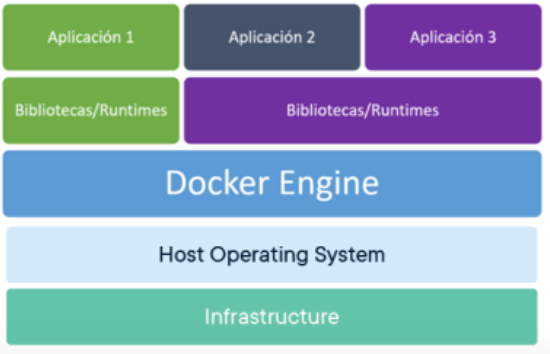
\includegraphics[width=0.7\textwidth]{imagenes/contenedores}
	\caption{Estructura de un sistema con contenedores}
	\label{fig:contenedores}
\end{figure}
	